\chapter{Context}
\label{chapter:context}

This chapter describes the context of this study. It starts by generally introducing the case company and its core businesses. After this
the focus is on software maintenance processes in the case company. After describing the processes, also the company focus points are presented to
clarify the initial motivational factors behind this study.

\section{Case company}
\label{section:case-company}

The case organization of this study is QOCO Systems Ltd., a small software company founded in 2009 focusing on
aviation industry with solid expertise in software solutions for maintenance, repair and operations (MRO) in aviation business.
During all of its lifespan there has been collaboration with Airline 1, which is still the most
important customer at the moment. A few years ago there was also quite much collaboration with a railway company since their
challenges with MRO were relatively similar to those of airlines. However, this collaboration has been discontinued due to
strategic focusing on the aviation market. At the start of this study, there were 16 employees at QOCO, which marks a 100 \% increase in 12 months.
Also the revenue has been growing steadily by around
200k\euro~ annually, currently being a bit over 1M\euro~ \citep{Finder.fi2019}. Basically it could be argued that QOCO is past the initial
startup phase as it has become a steadily profitable company with several employees and a solid customer base.

Main services offered by QOCO can be classified into two main categories: software services and consulting. During the last few years
consulting has been the most important revenue source for QOCO and therefore it still has a major role in QOCO's service portfolio.
Recently the main focus has been shifting towards Software as a Service (SaaS) business since consulting services require specialized expertise, making
them hard to scale up. SaaS solutions are selected as a strategical focus point because they can be scaled much easier and do not require as much in-depth technical
knowledge about aviation business, which is a relatively rare skill especially when combined with software development skills.

On the consulting side, QOCO's expertise is deeply focused on AMOS MRO System (AMOS), a system developed by Swiss AviationSoftware Ltd. and used
by many airlines worldwide for organizing their MRO processes. The main focus is on developing integrations between AMOS and various other systems,
but QOCO also provides support for data migration and several other AMOS related processes.

On the software solutions' side, QOCO has developed some SaaS solutions that are readily available for new customers. The portfolio consists mainly of
web applications and integrations, but QOCO has also worked with mobile applications in the past, however they are not the main focus area
at the moment. One example of a web application is MROTools.io, a tool management software meant for airlines to track the usage of tools during aircraft
maintenance and repair. Tool tracking is especially important in the aviation industry as a single missing tool could prevent an aircraft from departing
before it is found. On the integration services, QOCO has developed a data exchange service, EngineData.io, for automatic data transfer from aircraft
engines to the engine manufacturer's data analytics system so that it can be cross-checked with AMOS. The engine manufacturer's data analytics system then
calculates the wearing of different engine parts based on real measured values, which then can be used to plan the maintenance schedule according to actual wearing,
rather than using overly estimated values that are currently being used. This will optimize the maintenance schedule and increase the effective flight time of engines, which
will result in significant cost-savings over time. As the interface to the data analytics system is quite complex, QOCO has developed EngineData.io to hide the complexity,
making it much easier for the airlines to connect to the system and utilize its benefits.

The organization of QOCO is roughly divided into executives and four consulting and development teams. The executives include Managing Director, Chief Technology Officer (CTO),
Chief Customer Officer (CCO) and Chief Operating Officer (COO) and they are supervising the development and consulting teams. There is only one pure consulting
team consisting of two consultants allocated for Airline 1 and they are responsible for AMOS related migrations, reporting and other tasks typically related to
data engineering. Another team mainly on the consulting side, but more focused on developing highly tailored web applications and integrations is also allocated for Airline 1.
The team consists of one senior consultant that acts mostly as a product owner (PO) and is therefore ensuring that the team will constantly provide value for the customer by
prioritizing tasks and managing the communication between the team and the customer. In addition to the PO, there is also one senior and two junior developers
assigned to the team. There are also two product teams: one with four members focusing on MROTools and the other one with two members developing EngineData.
There are no separate POs in those teams, but
one of the executives will ensure that the product is developing into the right direction. The teams and their members are also presented in figure \ref{fig:organization}.

\begin{figure}[H]
	\begin{center}
		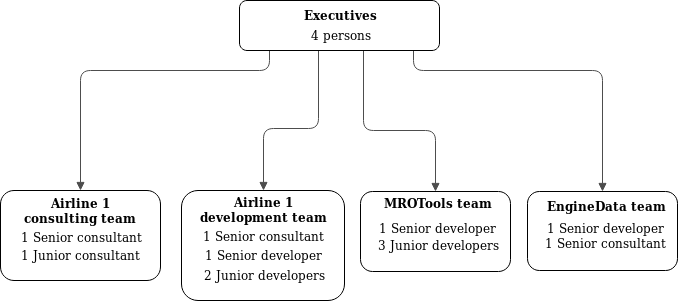
\includegraphics[width=.9\textwidth]{images/Organization}
		\caption{Organization structure as of January 2019}
		\label{fig:organization}
	\end{center}
\end{figure}

\section{Software maintenance in the case company}
As described, QOCO has grown rapidly during the last five years and that led to a point where the lack of a well defined software maintenance process was causing trouble
in day-to-day business and continuous interruptions made it difficult to focus on actual development tasks. Previously the maintenance process was based on directly contacting the contact person
via email or phone. Usually the contact person was the CTO who is also the founder of the company so he has a long background with the customers making him the most natural point of
contact for them. At the same time there were also new application management service (AMS) contracts being signed and those included requirements for response and resolution times
for example. Because of these new service level agreements (SLA), the previous "best effort" type of maintenance process could not be accepted anymore and a need for a well defined
maintenance process was identified.

As a core of the process improvement, QOCO decided to compare different options for issue tracking in spring 2017. A few requirements for the issue tracking system were identified:
most importantly it should be easy to use with a possibility for different contacting methods, including email and phone. It should also be reasonably priced for a group of 5 - 30 users
and it should support SLA modeling out of the box. Nice things to have in addition were support for reporting out of the box and grouping users by different customers, but these
were not considered as critical requirements. Five different issue tracking systems were evaluated in addition to considering implementing a custom integration for reporting incidents
directly to an internal issue tracking system. After a careful evaluation, QOCO chose Freshdesk out of its competitors to be taken into use in June 2017. Some key aspects
affecting the choice were its good quality for a reasonable price, ease of use and a good variety of out of the box features such as reporting and integrations to different
contacting methods. There is also a support for grouping users for different customers which improves its scalability in the long term if QOCO continues to grow as it has been
for the last few years.

In QOCO's case, maintenance activities can roughly be divided into two categories: general support and application management with further development. The maintenance
tasks vary between SaaS products and consulting services, because SaaS products are sold with the maintenance plan including further development
whereas consulting services are sold as a single delivery with a minimal support plan keeping the service up and running, but further development will always require new negotiations.
QOCO focuses mainly on in-depth technical support rather than providing basic user support such as password resetting.
This is mainly due to company's history of being a specialized consulting service provider for Airline 1 having only a few employees, which makes it
incapable of handling basic user support that would require dedicated customer service personnel.
Also the nature of services provided is deeply technical so there has not been a need for basic user support in a large scale. However due to the recent
strategic shift to providing products, like MROTools and EngineData, alongside with consulting has raised the demand for it, which also poses new
challenges for existing processes on scalability.

Currently there are two main channels to contact QOCO in case of incidents: a support email address for incidents that are not business critical and an emergency
phone number for critical incidents. In addition to these channels there are also some customers contacting their contact persons directly by email, mostly because of
the previous model that was based on direct contacts, but QOCO is trying to direct these requests to the official channels as well. Next both of the official channels are presented
in more detail.

\subsection{Support email address}

Support email address is used for low, medium and high priority incidents during the normal office hours. The process starts with a message to the support email address that
then automatically creates a ticket to Freshdesk with low priority and notifies relevant users by email. Relevant users are determined currently by certain domain rules,
mapping each customer to a group of Freshdesk users. After the notification, the ticket waits until someone will have a look on it and determine its priority, tasks to be done
and who will be addressing it. The ticket is then assigned for a consultant or a developer who will do the actual work. It is important to note that, depending on the issue,
this might be the same person that also did the prioritizing, but not in all cases as all of the developers and consultants do not have access to Freshdesk. The access is limited because
most of the incidents require further clarifications from the customer, which makes it natural for the contact person to handle the communication with the customer, letting the
developers and consultants focus on their work. After the clarifications, the contact person will then describe the issue for the consultant or developer who then can work
efficiently on resolving it.

During the resolution phase the assignee works on the issue and discusses about it with other team members and the contact person. In some cases there might be some further
information required from the customer or some third party, which will be shown as "waiting" status on Freshdesk meaning that QOCO's SLA timers are not running while waiting
for a response. When the issue gets resolved, its resolution is discussed with the customer and it will be agreed whether it requires any further actions to be taken. 

The whole process is presented in figure \ref{fig:ticketing}. As can be seen, the main interaction channel with the customer is the support email that will send notifications
to the customer if there are new comments added to the ticket. This way all of the information related to some incident is always
available on Freshdesk and not on someone's personal email account like it used to be in the previous model.

\begin{figure}[H]
	\begin{center}
		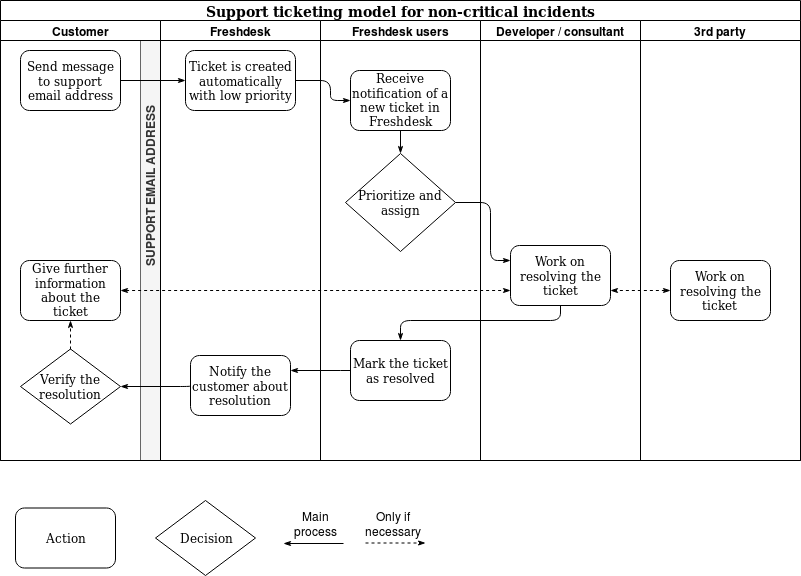
\includegraphics[width=.9\textwidth]{images/Current_support_process.png}
		\caption{Process for handling low, medium and high priority incidents}
		\label{fig:ticketing}
	\end{center}
\end{figure}

\subsection{Emergency phone}
In addition to the general support ticketing process, there is also an emergency phone number that the customers can call at any time. The emergency phone is meant only for
business critical issues that need to be dealt with immediately regardless of the time of day. This is crucial in aviation business as the business is operated in three shifts
24 hours a day, 7 days a week, and if the systems were to encounter critical incidents, they can not wait for the next morning before someone addresses them. This is why QOCO has
taken the emergency phone into use. It currently works as a service that first tries to redirect the call to the COO and if he does not answer, it will be redirected to the CTO and
the loop goes on until one of them picks the call. Due to nature of the incidents and their possible occurrence outside of normal office hours, QOCO's executives usually deal with
them alone without any need to involve other employees. However in some cases the developers and consultants might have particular expertise that helps to solve
the issue faster and thus they might provide some help if necessary. The process is presented in figure \ref{fig:emergency} and as can be seen, it is much more straightforward
compared to the normal process of handling low, medium and high priority incidents. However, the main process is still quite similar: the customer informs QOCO about the issue, QOCO deals with it and
discusses about the resolution with the customer who then verifies the resolution.

\begin{figure}[H]
	\begin{center}
		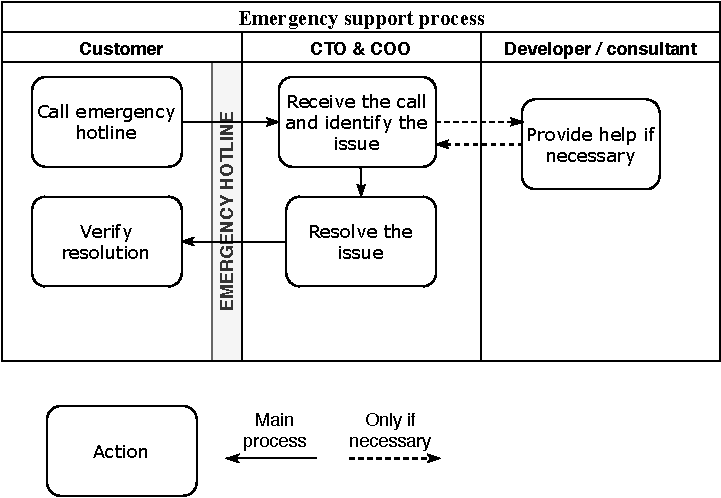
\includegraphics[width=.8\textwidth]{images/Emergency_support_process}
		\caption{Process for handling critical incidents}
		\label{fig:emergency}
	\end{center}
\end{figure}


\subsection{Application management and further development}
In addition to resolving incidents and providing support for customers when they ask for it, QOCO also has agreed to provide application management as a part of maintenance.
In general this means updating dependencies when necessary, monitoring capacities and reacting to alerts raised by crossing certain limits for example. In some cases the
alerts have been integrated with Freshdesk by sending automated messages to the support email address, which will then trigger the normal process for handling such incidents.
However the alerts are usually not integrated to Freshdesk right away and currently it is more like a nice additional feature rather than being required from the very beginning for each project,
which is a clear point of improvement. Other tasks such as updating the dependencies are also not addressed on a regular basis. Of course as QOCO follows the latest
discussion on its field, the version updates on relevant libraries and frameworks sometimes become a hot topic due to known vulnerabilities or support plans coming to an end. This then 
triggers the action on QOCO's side to take the necessary steps to keep the delivered software up to date to avoid those issues. Other than that, general updates to newer versions
of the dependencies occur in an unstructured way for example with new releases.

For further development part, the process is more open for different communication channels. Sometimes requests for new features or changes to existing ones are sent to
the support email address which then starts the process of incident handling. In those cases the ticket will be most likely closed in Freshdesk without further actions
and the requirements and schedule for the new feature are discussed with the customer outside of Freshdesk since it is not a support task that is meant to be handled in Freshdesk.
The requests can also be presented in meetings, by email or by phone directly to QOCO's personnel that then discusses and analyzes the requests in detail eventually agreeing about a development
plan with the customer. There are some differences between custom made consulting services and general products in terms of further development, the main difference
being that further development is usually already included in the maintenance plan for delivered products. This means that there is no need for additional discussions
about budgeting if the issue is estimated to fit into the agreed workload. On the consulting side, new features and changes to existing ones are not usually sold with the initial
contract that only covers the development of the first version and its support. This means that all requests need to be discussed with the customer to agree about the
budget and implementation schedule. This also makes it harder for QOCO to suggest new features that could generate more sales in the future.

\section{Company focus points}
\label{section:focus-points}

The key focus points for QOCO were identified in two separate interviews, first with the CTO, CCO and COO, the second with only CTO. The topics for those interviews were to
discuss about the current maintenance process, already identified issues with it and metrics that could represent the situation. The metrics would also be used to measure
the change after the implementation phase to see if the implemented solutions had any effect on the identified issues. During the first interview it was evident that the main
focus of the thesis should be on internal process improvements rather than having significant efforts on external processes that are more or less out of QOCO's reach.

One of the main problems already identified at this point was knowledge sharing, meaning that most of the maintenance tasks were handled by the CTO and COO without engaging
other personnel. This poses a risk as this way of working is not scalable in the future. It is assumed that there will be a growing amount of maintenance related
activities as the company matures and more and more projects are shifted to maintenance mode from active development leading to more serious problems in the future.
The fact that the CTO and COO handled most of the tasks
affected further sales and managerial activities that consume an increasing amount of time when the company grows and therefore maintenance knowledge needs to be shared
to other personnel as well. In addition to that, there was no clear responsibility for anyone to respond and resolve the newly created tickets, which easily leads to
a "someone will do it" attitude. This naturally causes further uncertainty on overall process and causes unnecessary delays.

Another important initial idea about the main challenges was the relationship between maintenance and development tasks. The overall feeling was that maintenance tasks
interrupt the development work, which results in frequent context switches slowing down both development and maintenance tasks. There was also a feeling that
this could be due to undefined process practices at least on some level, but at this point it could not be evaluated further in detail. One of the reasons for the
unstructured relationship between maintenance and development tasks was thought to be lack of a structured handover to the maintenance phase. On the other hand,
there is no separate maintenance personnel since the developers handle also maintenance of the developed systems, which explains the close relationship of different
tasks.

Customer satisfaction was also discussed in both interviews as it was identified to be important for the company. The initial thought was that customer satisfaction is
relatively good, which was based on an overall feeling and some interviews conducted a while ago. However a well defined metric to actually measure it was not defined and therefore
the initial feeling about a relatively good customer satisfaction was not based on any recent measurements. This was clearly a point of improvement although it was
considered to be less critical than internal process improvements.